\documentclass{subfiles}

\begin{document}

\textit{Cadeia de Markov} é um processo estocástico no qual a probabilidade do próximo estado depende apenas do estado anterior. Se o processo ainda tiver uma quantidade finita de estados e o tempo for discreto, é possível representar a cadeia como grafo direcionado completo como representado na Figura \ref{fig:auto_rep}. Cada estado corresponde a um nó do grafo, partindo de cada nó o estado seguinte é uma variável aleatória com as probabilidades representadas nos pesos de cada aresta. Por tanto, no caso ilustrado na Figura \ref{fig:auto_rep}
\begin{gather*}
	\text{Para todo } e, e^\prime \in E = \{A, B, C\} \\
	P(e^\prime|e) \in [0, 1] \text{ e }\\
	P(A|e) + P(B|e) + P(C|e) = 1
\end{gather*}
Como se espera de uma função probabilidade com domínio discreto. A partir do grafo é bastante direto representar os parâmetros de forma matricial
\[
    T = \begin{pmatrix}
        P(A|A) & P(B|A) & P(C|A) \\
        P(A|B) & P(B|B) & P(C|B) \\
        P(A|C) & P(B|C) & P(C|C)
    \end{pmatrix}
\]

Por outro lado, há redundâncias na matriz, pois cada linha soma $1$, por isso é suficiente $6$ parâmetros para determinar uma cadeia de $3$ estados. Além disso, existe uma distribuição de probabilidade para o valor inicial da sequência que será representado como $\pi_0(e)$ que é equivalente ao vetor
\[
	\Pi_0 = \begin{pmatrix}
		\pi_0(A) \\
		\pi_0(B) \\
		\pi_0(C)
	\end{pmatrix}
\]

De forma geral, em uma \textit{Cadeia de Markov} com $n$ estados, são necessários $n^2 - n$ parâmetros e cada probabilidade condicional é representada numa matriz $T \in \mathbb{R}^{n \times n}$ com entradas não negativas e que
\[
	T \mathbf{1}_n = \mathbf{1}_n
\]
Isto é, cada linha soma $1$. Além disso, também vetor $\Pi_0 \in \mathbb{R}^n$ com a distribuição de probabilidades para o estado inicial que também somam 1:
\[
	\Pi_0^{\mathrm T} \mathbf{1}_n = 1
\]
E da mesma forma que a matriz transição, à redundância no vetor $\Pi_0$, pois é suficiente determinar apenas as probabilidades de $n-1$ estados.

Concluí-se que uma \textit{Cadeia de Markov} de $n$ estados é definida por $n^2-1$ parâmetros.

\begin{figure} % Single column figure
	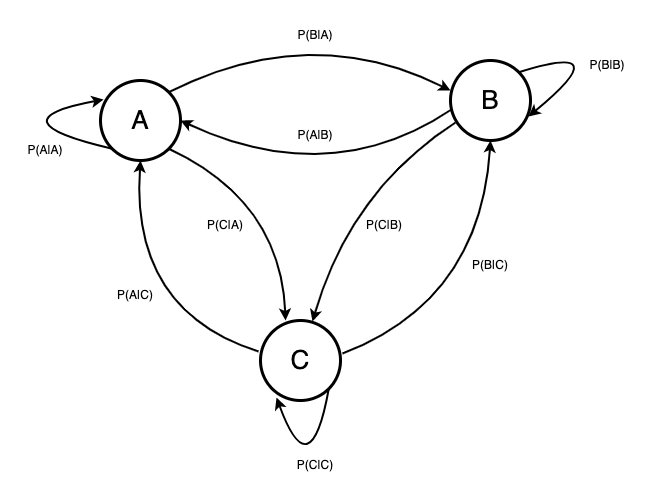
\includegraphics[width=\linewidth]{markov_chain.png}
	\caption{Diagrama de estados.}
	\label{fig:auto_rep}
\end{figure}

\subsection{Exemplo} \label{sub:exemplo}

Para ilustrar a estimativa dos parâmetros de uma \textit{Cadeia de Markov}, considere o seguinte conjunto sequências
\begin{align*}
	&ABCABACCACAB         \\
	&BACABACAAC           \\
	&BBABAAAACCACABABABAC
\end{align*}

Para estimar a matriz transição $T$, observe que, há no total que $20$ ocorrências da letra $A$ seguida de algum estado, $10$ da $B$, e $9$ da $C$. Ao se contar cada ocorrência das tuplas $AA$, $AB$, $AC$, e assim por diante, dividindo pela ocorrência do respectivo estado antecessor. Assim a seguinte matriz transição é obtida
\[
    \begin{pmatrix}
        \frac{4}{20} & \frac{8}{20} & \frac{8}{20} \\
        \frac{8}{10} & \frac{1}{10} & \frac{1}{10} \\
        \frac{7}{9} & \frac{0}{9} & \frac{2}{9}
    \end{pmatrix}
\]

Já para a estimativa do vetor probabilidade de estado inicial $\Pi_0$, o processo é imediato, é a frequência pela quantidade de sequências
\[
	\Pi_0 = \begin{pmatrix}
		\frac{1}{3} & \frac{2}{3} & 0
	\end{pmatrix}
\]

\subsection{Probabilidade Estacionária}

Agora suponha que algum processo é caracterizado como \textit{Cadeia de Markov} tenha matriz transição $T$, então note
\[
	(T - I)\mathbf{1} = T\mathbf{1} - I\mathbf{1} = \mathbf{1} - \mathbf{1} = O
\]
Isto é, tal matriz é $T - I$ não é linearmente independente e por tanto, tem determinante $0$. Isto implica que $1$ é autovalor da matriz $T$. Por tanto existe um vetor linha $V$ tal que
\[
	VT = V
\]
Como todas entradas de $T$ são não-negativas, $V$ só pode ter entradas não-negativas. Além disso, podemos multiplicar a igualdade por qualquer escalar em ambos os lados que a igualdade se mantém, por isso podemos forçar que $V\mathbf{1} = 1$. Chama-se $V$ de \textit{Probabilidade Estacionária}, isto é, a distribuição de probabilidade dos estados converge para $V$

\subsection{Modelos Alternativos}
Há também a possibilidade de expandir o modelo adicionando mais estados na dependência do estado seguinte, como Bishop\autocite{Bishop:2006pat} discute, mas isso vem com o custo de mais variáveis para se calcular. A medida que se adiciona $1$ estado na dependência, se multiplica a quantidade de parâmetros por $n$, a quantidade de estados.

Este nível de detalhamento pode tornar o modelo impraticável quando esta expansão se torna muito grande. Além disso, as estimativas dos parâmetros desse modelo passa depender de mais observações. Observe que não há ocorrências do par $CB$ no exemplo visto. Isto pode ter sido causado pelo fato de que o processo não permita essa transição de estado, mas também é possível que essa transição só não tenha sido observada na amostra apresentada.

\end{document}